O diâmetro do cabo é dado pela equação:

\begin{equation}
  d_c = Q\sqrt{T}
  \label{eq:diametro_do_cabo}
\end{equation}

Onde:

\begin{itemize}[leftmargin=1.25cm]
  \item $d_c$: diâmetro do cabo em $\si{\milli\meter}$.
  \item $Q$: coeficiente segundo a norma NBR 8400 \cite{nbr8400}.
  \item $T$: força de tração no cabo em $\si{\deca\newton}$.
\end{itemize}

\vspace{1em}

O coeficiente Q foi obtido na tabela 27 da NBR 8400 \cite{nbr8400}:

\begin{figure}[H]
  \centering
  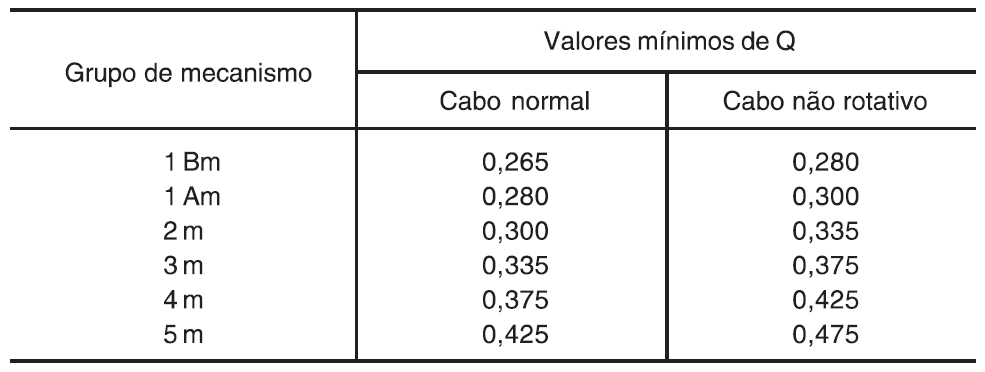
\includegraphics[width=0.5\textwidth]{content/sections/03_sistema_de_elevacao/sections/04_diametro_do_cabo/images/coeficiente_q.png}
  \caption{Valores Mínimos de Q \cite{nbr8400}}
  \label{fig:coeficiente_q}
\end{figure}

Para o grupo de mecanismo 1AM, o valor de $Q$ para cabo normal é $0,28$.

\vspace{1em}

Substituindo os valores na equação \eqref{eq:diametro_do_cabo}:

\begin{align*}
  d_c & = 0,28 \sqrt{2537,78}              \\
  d_c & = \boxed{\SI{14,11}{\milli\meter}}
\end{align*}

Adotou-se um cabo de aço CIMAF, classe 6x41 Warrington-Seale IPS, com alma de fibra. As propriedades do cabo, conforme o catálogo da CIMAF \cite{cimaf_cabos_aco}, são:

\begin{figure}[H]
  \centering
  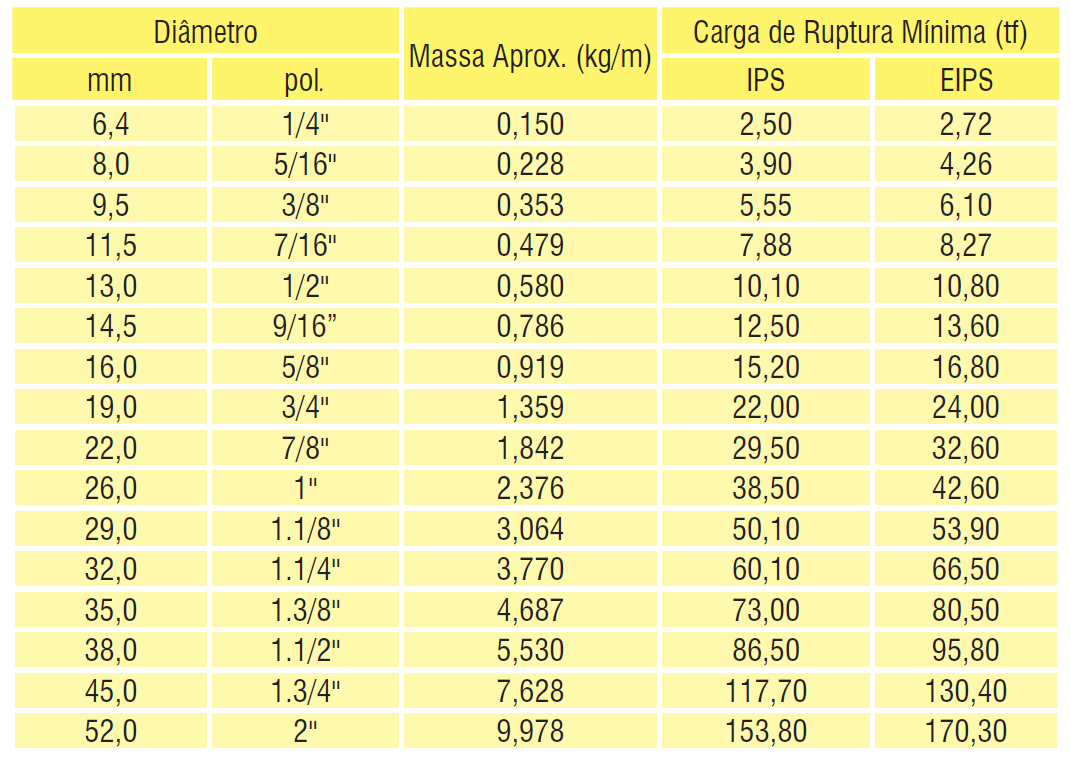
\includegraphics[width=0.5\textwidth]{content/sections/03_sistema_de_elevacao/sections/04_diametro_do_cabo/images/propriedades_cabos_cimaf.png}
  \caption{Propriedades dos cabos de aço da CIMAF \cite{cimaf_cabos_aco}}
  \label{fig:propriedades_cabos_cimaf}
\end{figure}

Para um cabo de \SI{14,5}{\milli\meter}, a carga de ruptura mínima é de \SI{12,5}{\tonneforce}.

Segundo o catálogo da CIMAF \cite{cimaf_cabos_aco}, o fator de segurança deve ser de $6$ a $8$ para pontes rolantes, aplicável também a pórticos rolantes. Os valores recomendados são:

\begin{figure}[H]
  \centering
  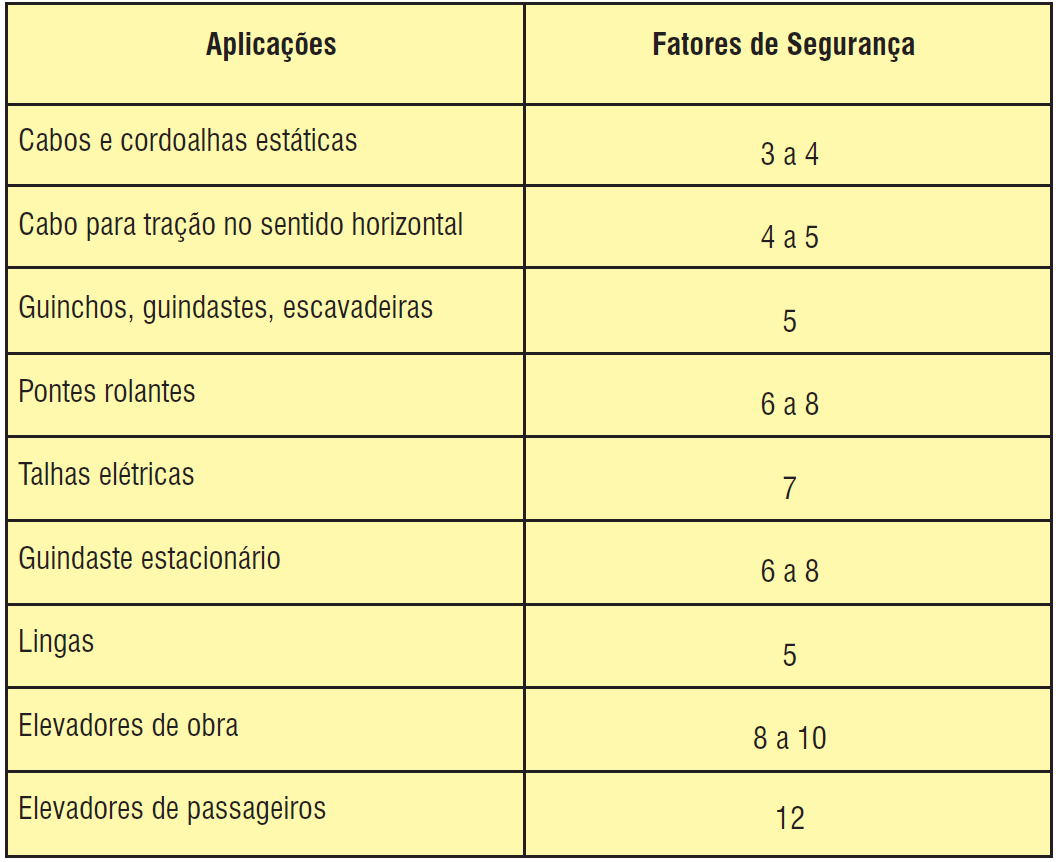
\includegraphics[width=0.5\textwidth]{content/sections/03_sistema_de_elevacao/sections/04_diametro_do_cabo/images/fator_seguranca_cimaf.png}
  \caption{Fatores de segurança da CIMAF \cite{cimaf_cabos_aco}}
  \label{fig:fator_seguranca_cimaf}
\end{figure}

No catálogo da CIMAF \cite{cimaf_cabos_aco}, o fator de segurança é definido pela seguinte equação:

\begin{equation}
  F_s = \frac{CRM}{T}
  \label{eq:fator_seguranca}
\end{equation}

Onde:

\begin{itemize}[leftmargin=1.25cm]
  \item $F_s$: fator de segurança.
  \item $CRM$: carga de ruptura mínima em $\si{\tonneforce}$.
  \item $T$: força de tração no cabo em $\si{\tonneforce}$.
\end{itemize}

\vspace{1em}

Substituindo os valores na equação \eqref{eq:fator_seguranca}:

\begin{align*}
  F_s & = \frac{12,5}{2537,78 \cdot 10^{-3}}       \\
  F_s & = 4,93 \leq 6 \rightarrow \text{Reprovado}
\end{align*}

O cabo adotado não atende aos requisitos de segurança; portanto, foi necessário selecionar um cabo de maior diâmetro. Adotou-se um cabo com diâmetro de \SI{16}{\milli\meter}, cuja carga de ruptura mínima é \SI{15,2}{\tonneforce}.

Aplicando a nova carga de ruptura mínima na equação \eqref{eq:fator_seguranca}:

\begin{align*}
  F_s & = \frac{15,2}{2537,78 \cdot 10^{-3}}       \\
  F_s & = 5,99 \leq 6 \rightarrow \text{Reprovado}
\end{align*}

O cabo adotado ainda não atende aos requisitos de segurança; assim, foi necessário selecionar um cabo de maior diâmetro. Adotou-se um cabo com diâmetro de \SI{19}{\milli\meter}, cuja carga de ruptura mínima é \SI{22}{\tonneforce}.

Aplicando a nova carga de ruptura mínima na equação \eqref{eq:fator_seguranca}:

\begin{align*}
  F_s & = \frac{22}{2537,78 \cdot 10^{-3}}   \\
  F_s & = \boxed{8,67} \geq 6 \rightarrow OK
\end{align*}

O cabo adotado atende aos requisitos de segurança.

\begin{table}[H]
  \centering
  \caption{Propriedades do cabo adotado}
  \begin{tabularx}{\textwidth}{>{\centering\arraybackslash}X>{\centering\arraybackslash}X>{\centering\arraybackslash}X}
    \toprule
    Parâmetro               & Símbolo           & Valor                         \\
    \midrule
    Diâmetro do cabo        & $d_c$             & \SI{19}{\milli\meter}         \\
    Massa por metro do cabo & $m_{\text{cabo}}$ & \SI{1,359}{\kilo\gram/\meter} \\
    Carga de ruptura mínima & $CRM$             & \SI{22}{\tonneforce}          \\
    \bottomrule
  \end{tabularx}
\end{table}
